\documentclass[tikz]{standalone}

\usetikzlibrary{cd}
\usetikzlibrary{arrows}
\usepackage{amsfonts,amssymb}
\usepackage{mathtools}
\usepackage{adjustbox}
\usetikzlibrary{decorations.pathmorphing}
\usetikzlibrary{decorations.markings}
\usetikzlibrary{arrows.meta,bending}





\def\ellipse{
	\adjustbox{scale=0.25}{%
		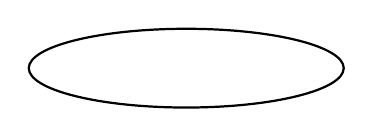
\begin{tikzpicture}
			\draw[thick] (0,0) ellipse (2cm and 0.5cm);
		 \end{tikzpicture}
	}
}
\def\helix{
	\adjustbox{scale=0.25}{%
		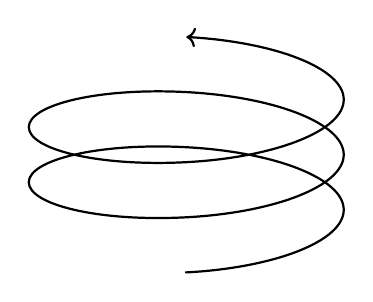
\begin{tikzpicture}
			\draw[thick,decoration={aspect=0.31, segment length=7mm,
		     amplitude=2cm,coil},decorate,arrows = {<[bend]-}] (0,4) --(0,1);
		 \end{tikzpicture}
	}
}


\begin{document}
	\begin{tikzcd}[row sep=scriptsize, column sep=scriptsize]
		\mathbb{Z} \ar[rr] \ar[dd] \ar[dr,"\mathclap{\sim}",sloped]& & \mathbb{R} \ar[dd] \ar[dr,"\mathclap{\sim}",sloped]& & \helix \ar[dd,mapsto]
		\\
		& \ast \ar[rr,crossing over] & & \ast \ar[dd] &
		\\
		\ast \ar[rr]  \ar[dr,"\mathclap{\sim}",sloped,equal]& & S^1 \ar[dr,"\mathclap{\sim}",sloped,equal] & & \ellipse
		\\
		& \ast \ar[from=uu,crossing over] \ar[rr]& & S^1 &
	\end{tikzcd}
\end{document}